% STYLE

	% DOCUMENT TYPE & GEOMETRY

\documentclass[11pt, english]{article}

        \usepackage{geometry}
                \geometry{
                        a4paper,total={210mm,297mm},
                        tmargin=40.8mm,
                        bmargin=40.8mm,
                        lmargin=32.6mm,
                        rmargin=32.6mm,
                }

        % Change font
        %\usepackage[T1]{fontenc}
        %\usepackage{CormorantGaramond}

        % Latin grammar pack
        \usepackage{tipa}

        % Page header formatting
        \usepackage{fancyhdr}
        \usepackage{lipsum}
                \pagestyle{fancy}
                \fancyhf{} % Removes default header and footer content
                \fancyhead[L]{\leftmark} % Leftmark header left (current section) (rightmark is current subsection)
                \fancyhead[R]{\thepage} % Page number header right
                \fancyfoot[C]{\thepage} % Page number footer center
                \renewcommand{\headrulewidth}{0.5pt} % Rule along header

	% Links
        \usepackage{hyperref} 
                \hypersetup{          
                        colorlinks=true,        
                        linkcolor=black,  
                        filecolor=magenta,
                        urlcolor=cyan,
                        }

	% TABLE OF CONTENTS, LIST OF TABLES, LIST OF FIGURES

        \usepackage{tocloft}
                
                % Style titles of ToC, LoT and LoF
                \renewcommand{\cfttoctitlefont}{\fontsize{18}{16}\scshape}
                \renewcommand{\cftlottitlefont}{\fontsize{18}{16}\scshape}
                \renewcommand{\cftloftitlefont}{\fontsize{18}{16}\scshape}

                % Style contents of ToC, LoT and LoF
                \renewcommand{\cftsecfont}{\scshape}
                \renewcommand{\cftsubsecfont}{\scshape}
                \renewcommand{\cftsubsubsecfont}{\scshape}
                \renewcommand{\cftparafont}{\scshape}

	% ABSTRACT TITLE

        \usepackage{abstract}
                \renewcommand{\abstractnamefont}{\fontsize{11}{0}\scshape}

	% SECTION TITLES & HEADINGS

        \renewcommand{\thesection}{\arabic{section}}
        \renewcommand{\thesubsection}{\thesection.\arabic{subsection}}
        \renewcommand{\thesubsubsection}{\thesubsection.\arabic{subsubsection}}
        \renewcommand{\theparagraph}{\thesubsubsection.\arabic{paragraph}}

        % Syntax section titles and headings
        \usepackage{titlesec}

                \titleformat{\section}
			{\fontsize{18}{16}\scshape}{\thesection}{0.5em}{} % Can do: {Text \thesection}, also {\bfseries} etc.

                \titleformat{\subsection}
                        {\fontsize{14}{16}\scshape}{\thesubsection}{1em}{}

                \titleformat{\subsubsection}
                        {\fontsize{11}{16}\scshape}{\thesubsubsection}{1em}{}

                % Redefining paragraph to 4th class section like '\subsubsubsection'
                \titleformat{\paragraph}
                        {\fontsize{11}{16}\scshape}{\theparagraph}{1em}{}

	% BODY TEXT & SOME SYNTAX

        % Removing paragraph indent
        \setlength{\parindent}{0pt}

        % Line stretch 
        \renewcommand{\baselinestretch}{1.25}
        % Allow varying intervals of line-width change
        \usepackage{setspace}

        % Defining new ruled line
        \newcommand{\HRule}[1]{\rule{\linewidth}{#1}}
                \setcounter{tocdepth}{5}
                \setcounter{secnumdepth}{5}

	% GRAPHICS

        \usepackage{graphicx}
        % Path to graphics
        \graphicspath{{./dir/}}

	% TABLES & FIGURES

        \usepackage{float}

        \usepackage{longtable}
        \usepackage{multicol}
        \usepackage{multirow}

        % Caption style
	\usepackage{caption} % Could use the captionsetup definitions in [] in this if lazy
		\captionsetup[table]{labelfont=sc,textfont=sc,font=small,skip=8pt}
		\captionsetup[figure]{labelfont=sc,textfont=sc,font=small,skip=8pt}
	\usepackage{subcaption}
		\captionsetup[subtable]{justification=raggedright,labelfont=sc,textfont=sc,font=small,skip=8pt,labelformat=parens,labelsep=space}
		\captionsetup[subfigure]{justification=raggedright,labelfont=sc,textfont=sc,font=small,skip=8pt,labelformat=parens,labelsep=space}

	% Table caption syntax
        \renewcommand{\thetable}
                {\thesection.\arabic{table}}
	\renewcommand{\thesubtable}
                {\roman{subtable}}

        % Figure caption syntax
        \renewcommand{\thefigure}
                {\thesection.\arabic{figure}}
	\renewcommand{\thesubfigure}
                {\roman{subfigure}}

	% MATH AND SYMBOLS

        \usepackage{amsmath}
        \usepackage{amssymb}

	% Trees
	\usepackage{tikz}
                \usetikzlibrary{trees,arrows,topaths}

	% BIBLIOGRAPHY

	% Enabling changes to be made to BibTeX title
        \usepackage{babel}

% DOCUMENT

\begin{document}

	\title{
                \HRule{0.5pt}\\[0.3cm]
                \huge\textsc{Article Title Class 1}\\
                \Large\textsc{Article Title Class 2}\\[0.25cm]
                \HRule{0.5pt}
                }
        \author{\textsc{Name}\\
                \textsc{Additional}\\
                \textit{Additional}
                }
        \date{}
	\maketitle

	\begin{center}
		\textsc{Article Title Class 3}
	\end{center}

	\vspace\fill

	\begin{center}
		\textit{Additional}
	\end{center}

	\begin{center}
		\fbox{\textsc{Boxed Text}}
	\end{center}

	\begin{center}
		\textsc{Additional}
	\end{center}

\newpage
% Abstract

% Lower-case roman numerals for prceeding text
\pagenumbering{roman}

	\begin{abstract}
		This is a sentence of text in the abstract.
	\end{abstract}

\newpage
% Table of Contents

	\renewcommand{\contentsname}{Table of Contents}

	\tableofcontents

\newpage
% List of Tables

	\listoftables

\newpage
% List of Figures

	\listoffigures

\newpage
% Body of text

% Arabic numerals for body text
\pagenumbering{arabic}

\section{Section Title}

	\subsection{Subsection Heading}

	\subsubsection{Subsubsection Heading}

	\paragraph{Paragraph Heading}

	\newpage

	This is a paragraph of text.\\

	\textbf{This is a paragraph of bold text.}\\

	\textit{This is a paragraph of italic text.}\\

	\textsl{This is a paragraph of slanted text.}\\

	\textsc{This is a paragraph of small-caps text.}\\

	\texttt{This is a paragraph of monospaced text.}

	\newpage 

	Basic unordered list:	

	\begin{itemize}
	% Additional spacing between items = 0
	\setlength\itemsep{0cm}
		\item Item using default first class
		\begin{itemize}
			\item Item using default second class
			\begin{itemize}
				\item Item using default third class
				\begin{itemize}
					\item Item using default fourth class
				\end{itemize}
			\end{itemize}
		\end{itemize}
	\end{itemize}

	Basic ordered list:

	\begin{enumerate}
	\setlength\itemsep{0cm}
                \item Item using default first class
                \begin{enumerate}        
                        \item Item using default second class
                        \begin{enumerate}
                                \item Item using default third class
                                \begin{enumerate}
                                        \item Item using default fourth class
                                \end{enumerate}   
                        \end{enumerate}
                \end{enumerate}
        \end{enumerate}

	Basic custom unordered list (using itemize):

	\begin{itemize}
	\setlength\itemsep{0cm}
		\item[$\alpha$] Item using custom first class
		\item[$\Longrightarrow$] Item using custom first class
		\item[$\blacksquare$] Item using custom first class
		\item[$\square$] Item using custom first class
        \end{itemize}

	\newpage

	Graphics:

	\begin{center}
                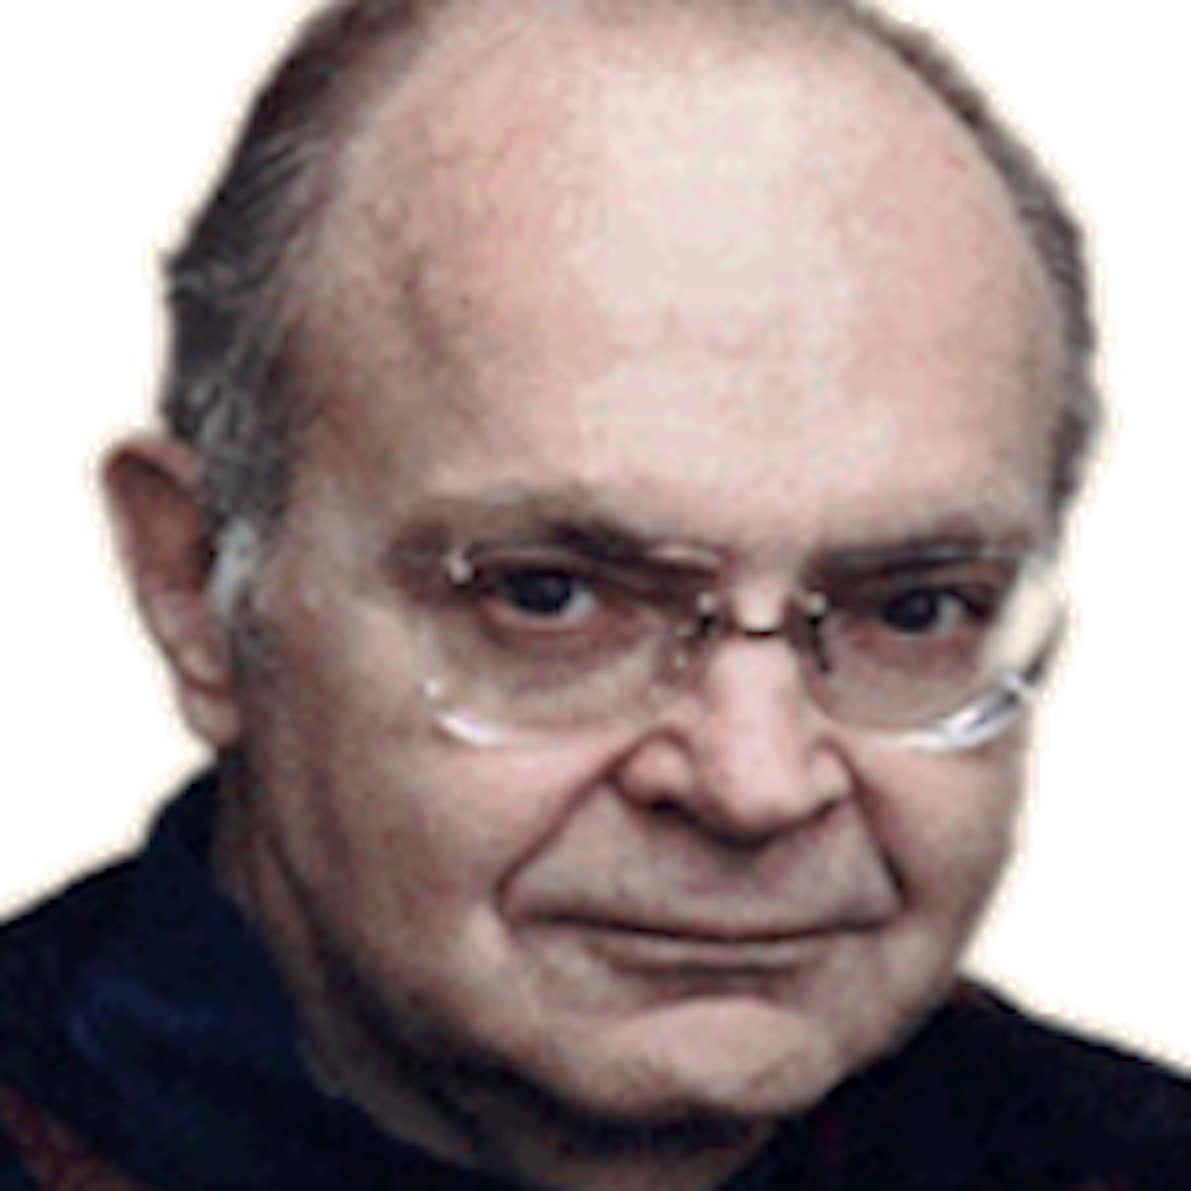
\includegraphics[width=8cm,height=6cm]{../Blog/Photos_FF/knuth.png}
        \end{center}

	\newpage

	Basic tabular:

	\begin{center}
                \small
        \begin{tabular}{r|l}
                \textsc{Mail To:} wi.lbritton@yahoo.com & \textsc{Telephone:} 07425 212 056\\
                \textsc{Website:} \href{http://lewisbritton.com}{lewisbritton.com} & \textsc{GitHub:} \href{https://github.com/FedeRog1977}{FedeRog1977}\\
        \end{tabular}
        \end{center}

	Basic table: 
	% Must use separate arraystretch to align with global document spacing

	\begin{table}[h]
		\scriptsize
		\renewcommand{\arraystretch}{1.25}
	\begin{center}
	\begin{tabular}{p{3cm}|p{2cm}p{2cm}p{2cm}p{2cm}}
		\hline
		\hline
		\multicolumn{5}{c}{Heading}\\
		\hline
		\hline
		\multicolumn{5}{c}{Heading 2}\\
		\hline
		\multirow{2}{*}{Word} & \multicolumn{4}{c}{Word}\\
		\cline{2-5}
		& Word & Word & Word & Word\\
		\hline
		Word & Value & Value & Value & Value\\
                Word & Value & Value & Value & Value\\
                Word & Value & Value & Value & Value\\
                Word & Value & Value & Value & Value\\
		\hline
		Word & \multicolumn{4}{l}{Left-aligned collective value}\\
		Word & \multicolumn{4}{r}{Right-aligned collective value}\\
		Word & \multicolumn{4}{c}{Centre-aligned collective value}\\
		\hline
		\hline
		\multicolumn{5}{c}{Heading}\\
		\hline
		\hline
		\multicolumn{5}{p{11.5cm}}{Some text in a paragraph.\newline Some more text in a paragraph, on a new line.}\\
		\hline
	\end{tabular}
		\caption{Table Caption}
	\end{center}
	\end{table}

	Basic longtable:
	% [1] Remove table, [2] repace tabular with longtable, [3] move formatting commands inside centre, [4] move caption inside longtable, [5] remove any arraystretch as longtable uses global stretch

        \begin{center}
                \scriptsize
        \begin{longtable}{p{3cm}|p{2cm}p{2cm}p{2cm}p{2cm}}
                \hline
                \hline
                \multicolumn{5}{c}{Heading}\\
                \hline
                \hline                 
                \multicolumn{5}{c}{Heading 2}\\
                \hline
                \multirow{2}{*}{Word} & \multicolumn{4}{c}{Word}\\
                \cline{2-5}                  
                & Word & Word & Word & Word\\
                \hline
                Word & Value & Value & Value & Value\\
                Word & Value & Value & Value & Value\\
                Word & Value & Value & Value & Value\\
                Word & Value & Value & Value & Value\\
                \hline
                Word & \multicolumn{4}{l}{Left-aligned collective value}\\        
                Word & \multicolumn{4}{r}{Right-aligned collective value}\\        
                Word & \multicolumn{4}{c}{Centre-aligned collective value}\\                                     
		\hline                                                                           
                \hline
                \multicolumn{5}{c}{Heading}\\
                \hline
                \hline                                                                                           
		\multicolumn{5}{p{11.5cm}}{Some text in a paragraph.\newline Some more text in a paragraph, on a new line.}\\                                               
                \hline                 
                \caption{Table Caption}
        \end{longtable}                
        \end{center}

	\newpage

	Table with subtables:

	\begin{table}[h]
	\begin{center}
		\begin{subtable}[t]{4cm}
		\begin{center}
		\begin{tabular}{|l|l|l|}
			\hline
			Value & Value & Value\\
			\hline
			Value & Value & Value\\
			\hline
		\end{tabular}
			\caption{Table Subcaption}
		\end{center}
		\end{subtable}
	\quad
		\begin{subtable}[t]{4cm}
		\begin{center}
		\begin{tabular}{|l|l|l|}
			\hline
			Value & Value & Value\\
			\hline
			Value & Value & Value\\
			\hline
		\end{tabular}
			\caption{Table Subcaption}
		\end{center}
		\end{subtable}
	\end{center}
		\caption{Table Caption}
	\end{table}

	\newpage

	Figure containing graphics:

	\begin{figure}[H]
	\begin{center}
		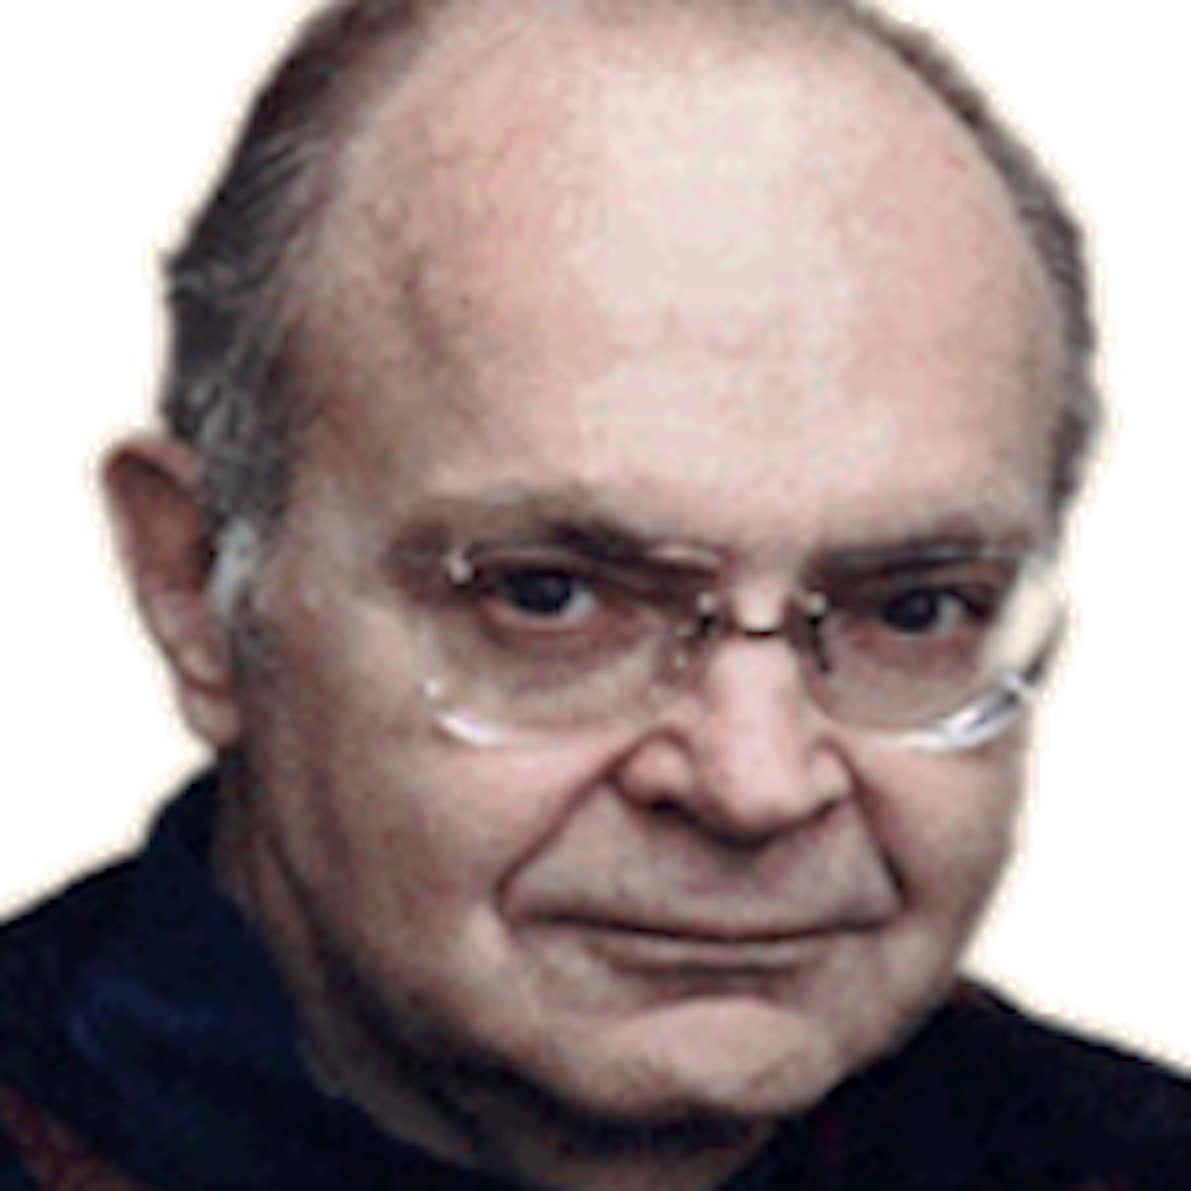
\includegraphics[width=8cm,height=6cm]{../Blog/Photos_FF/knuth.png}
		\caption{Figure Caption}
	\end{center}
	\end{figure}

	Figure with subfigures containing graphics:

	\begin{figure}[H]
	\begin{center}
		\begin{subfigure}[t]{5cm}
		\begin{center}
			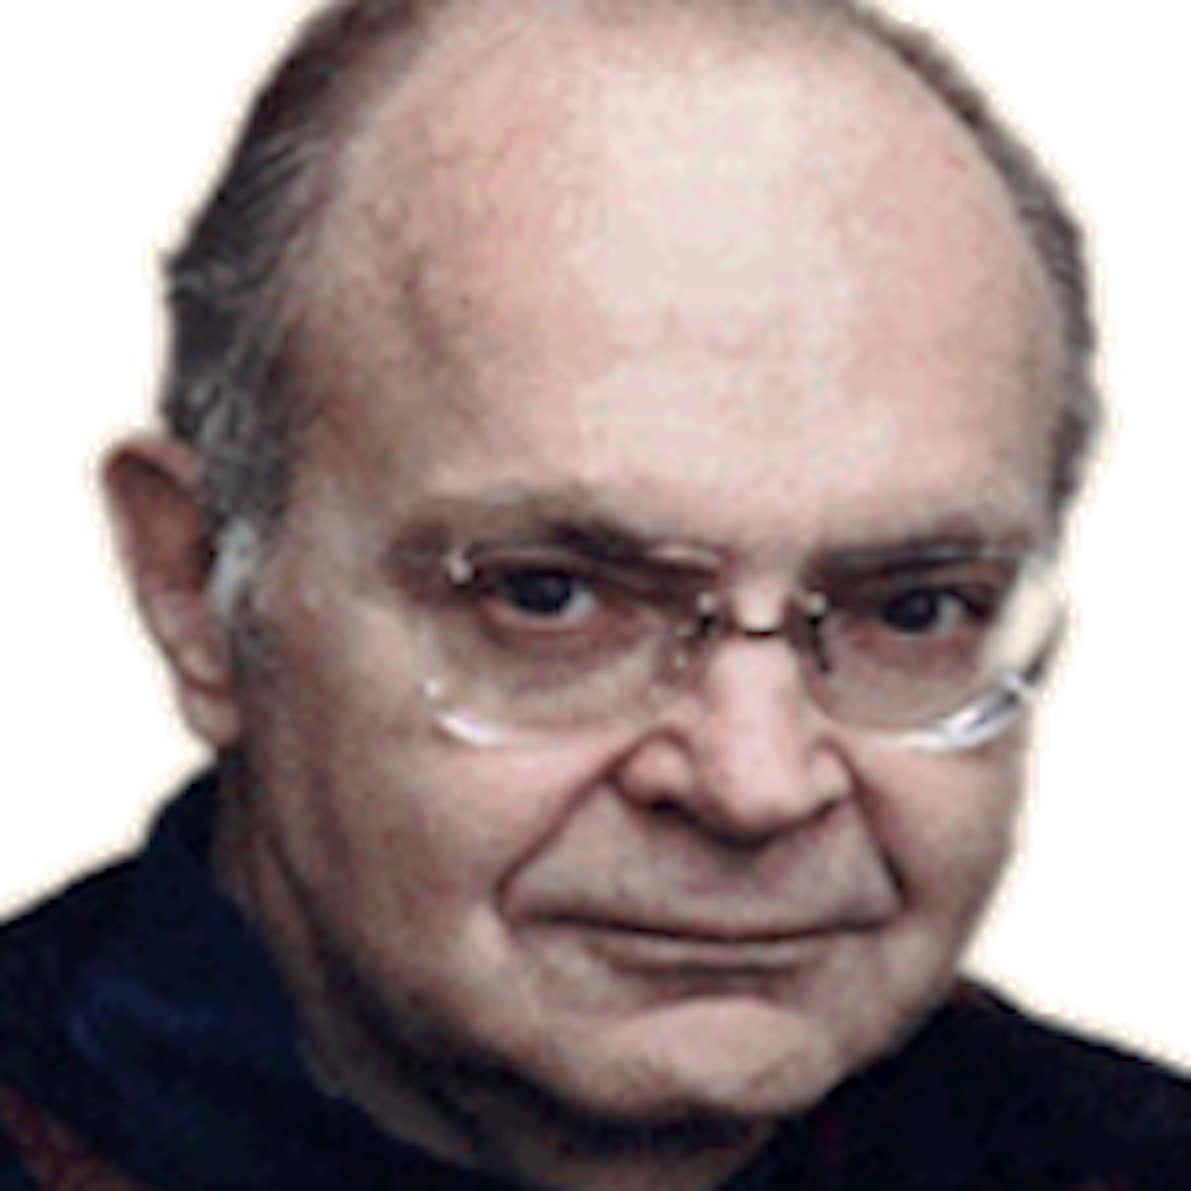
\includegraphics[width=4cm,height=3cm]{../Blog/Photos_FF/knuth.png}
		\end{center}
			\caption{Figure Subcaption}
		\end{subfigure}
                \begin{subfigure}[t]{5cm}
                \begin{center}
                        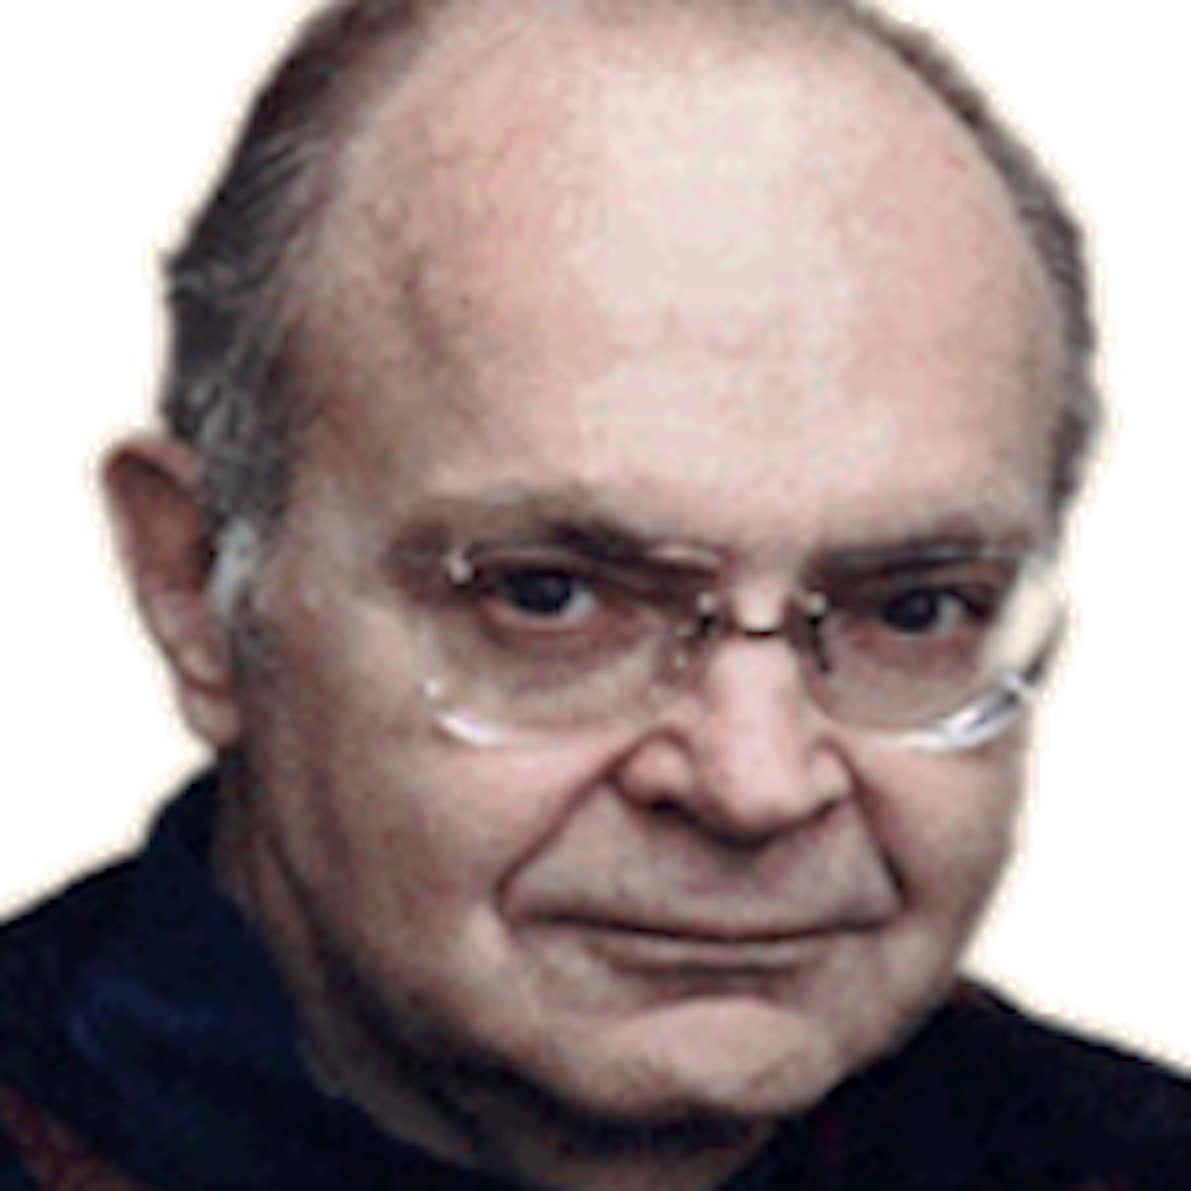
\includegraphics[width=4cm,height=3cm]{../Blog/Photos_FF/knuth.png}
                \end{center}
                        \caption{Figure Subcaption}
                \end{subfigure}
	\quad
		\begin{subfigure}[t]{5cm}
		\begin{center}
			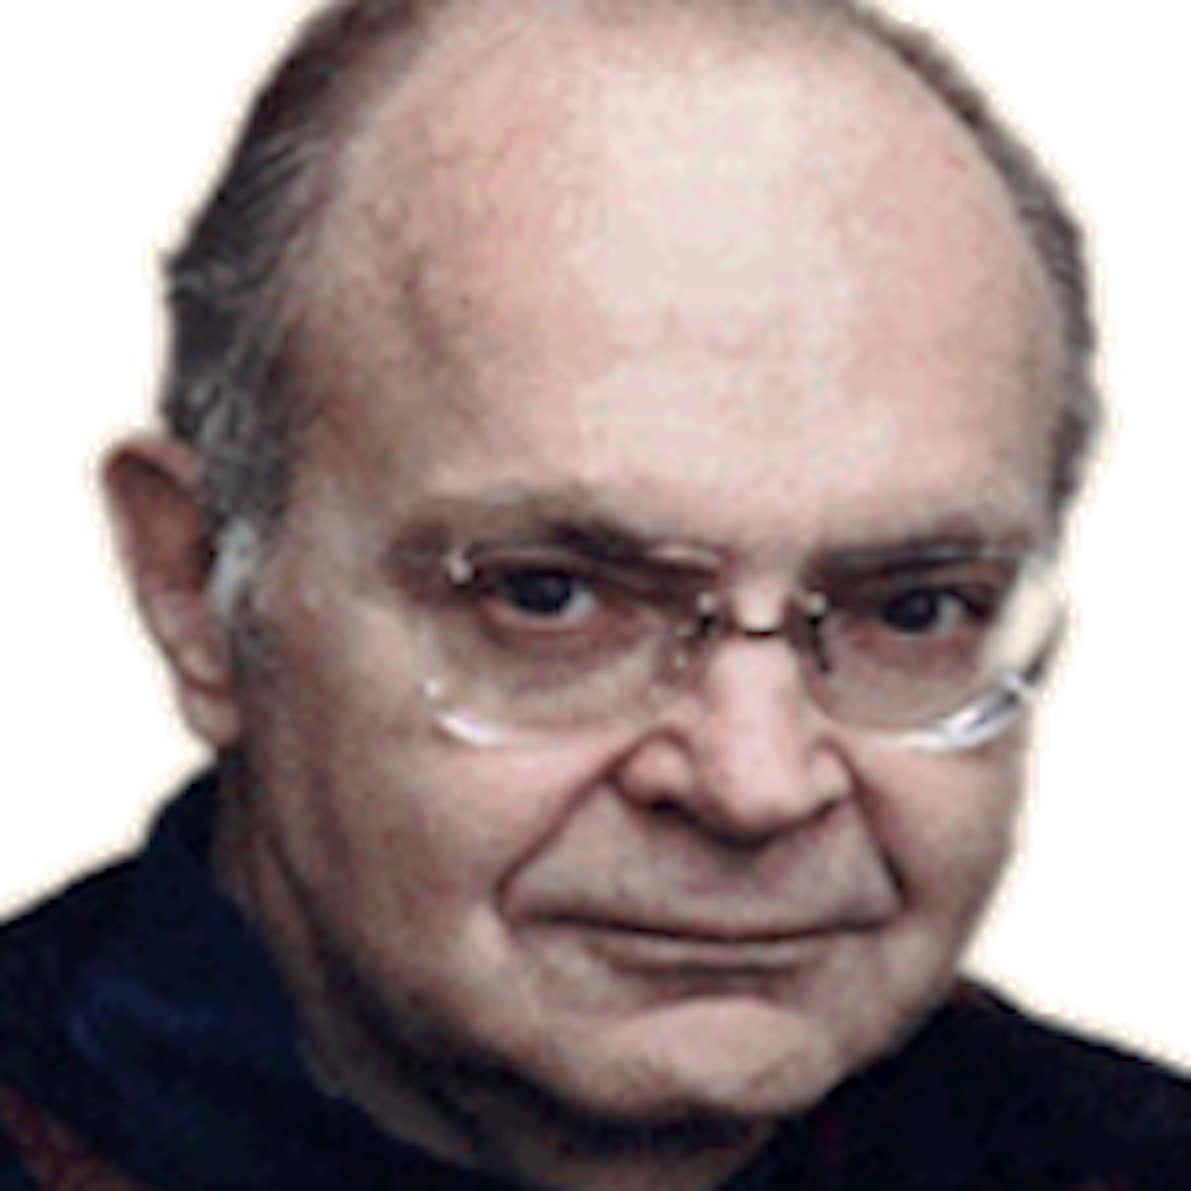
\includegraphics[width=4cm,height=3cm]{../Blog/Photos_FF/knuth.png}
		\end{center}
			\caption{Figure Subcaption}
		\end{subfigure}
                \begin{subfigure}[t]{5cm}
                \begin{center}
			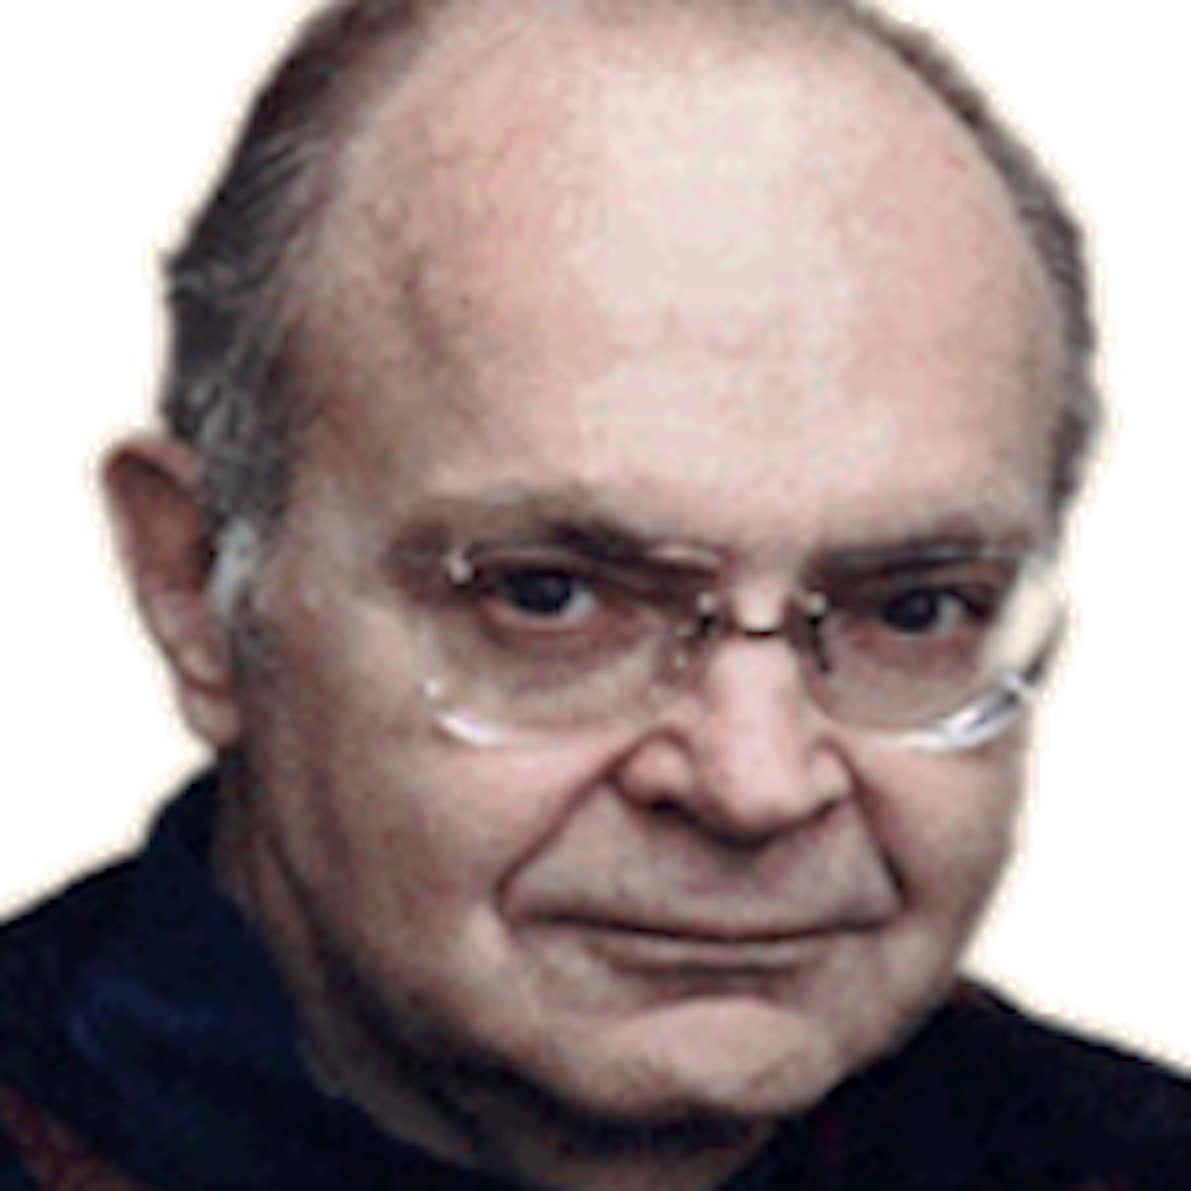
\includegraphics[width=4cm,height=3cm]{../Blog/Photos_FF/knuth.png}
                \end{center}
                        \caption{Figure Subcaption}
                \end{subfigure}
	\end{center}
		\caption{Figure Caption}
	\end{figure}

	\newpage

	Math mode:

	$$x=\frac{-b\pm\sqrt{b^2-4ac}}{2a}$$

	Math mode in-line:\\

	$a=Standard\ Text$\\
	$b=\mathrm{Roman\ Text}$\\
	$c=\mathit{Italic\ Text}$\\
	$x=\mathbf{Bold\ Face\ Text}$
	
	\newpage

	Vertical (recursion) tree (Ti\textit{k}Z package):\\

	\tikzstyle{level 1}=[level distance=2cm, sibling distance=8cm]
        \tikzstyle{level 2}=[level distance=2cm, sibling distance=4cm]

	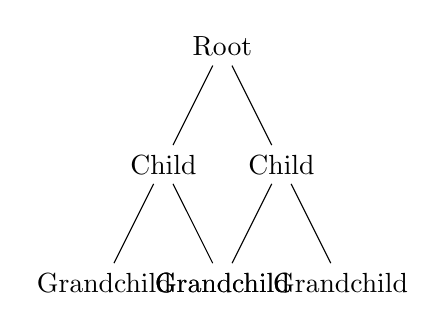
\begin{tikzpicture}
		\node {Root}
			child {
				node {Child}
					child {
						node {Grandchild}
						}
                                	child {
						node {Grandchild}
						}
				}
			child {
				node {Child}
					child {
						node {Grandchild}
						}
					child {
						node {Grandchild}
						}
				};
	\end{tikzpicture}\\

	Horizontal (probability) tree (Ti\textit{k}Z package):\\

	\tikzstyle{level 1}=[level distance=6cm, sibling distance=6cm]
        \tikzstyle{level 2}=[level distance=6cm, sibling distance=4cm]

        \tikzstyle{bag} = [text width=3em, text centered]
        \tikzstyle{end} = [text width=3em, text centered]

        \begin{tikzpicture}[grow=right, sloped]
		\node[bag] {Root}
                	child {
				node[bag] {Child}
	                		child {
						node[end] {Grandchild}
                	                	edge from parent
                	                	        node[above] {} % Text above line
                	                	        node[below] {} % Text below line
                	                	}
                	        	child {
						node[end] {Grandchild}
                	        	        edge from parent
                	        	                node[above] {}
                	        	                node[below] {}
                	        	        }
                	        	        edge from parent 
							node[above] {}
							node[below] {}
                	        }
                	child {
				node[bag] {Child}
                	        	child {
						node[end] {Grandchild}
                	        	        edge from parent
							node[above] {}
							node[below] {}
                	        	        }
                	        	child {
						node[end] {Grandchild}
                	        	        edge from parent
							node[above] {}
							node[below] {}
                	        	        }
                	        	        edge from parent         
							node[above] {}
							node[below] {}
                	        };
        \end{tikzpicture}

\newpage      

        Bibliography using simplest of the simple \textsc{Bib}{\TeX} syntax:

\renewcommand\refname{Bibliography}
                          
\begin{thebibliography}{9}                                                                                                                           
                                                                                                                                                    
        \bibitem{a}                                                                                                                                 
                Surname, Forename Initial., Surname, Forename Initial. (YYYY).
                \textsl{Article Title.}                                
                Publisher / Institution, Volume, Issue, Page Number(s).

	\bibitem{b}                                                                                                                                 
                Surname, Forename Initial., Surname, Forename Initial. (YYYY).
                \textsl{Article Title.}                                
                Publisher / Institution, Volume, Issue, Page Number(s).
	
	\bibitem{c}                                                                                                                                 
                Surname, Forename Initial., Surname, Forename Initial. (YYYY).
                \textsl{Article Title.}                                
                Publisher / Institution, Volume, Issue, Page Number(s).

	\bibitem{d}                                                                                                                                 
                Surname, Forename Initial., Surname, Forename Initial. (YYYY).
                \textsl{Article Title.}                                
                Publisher / Institution, Volume, Issue, Page Number(s).

\end{thebibliography}

\newpage

\pagenumbering{gobble}

	No page number.

\newpage 

\pagenumbering{arabic}

	Arabic page number.

\newpage

\pagenumbering{alph}

	Lower-case alphabetical page number.

\newpage 

\pagenumbering{Alph}

	Upper-case alphabetical page number.

\newpage

\pagenumbering{roman}

	Lower-case roman page number.

\newpage

\pagenumbering{Roman}

	Upper-case roman page number.

\end{document}
